%%%%%%%%%%%%%%%%%%%%%%%%%%%%%%%%%%%%%%%%%%%%%%%%%%%%%%%%%%%%%%%%%%%%%%%%%%%%%%%%%%%%%%
% This LaTeX file was prepared by:
%       Rajat Subhra Chakraborty
%       Assistant Professor
%       Dept. of Computer Science and Engineering
%       IIT Kharagpur
%       Kharagpur, India - 721302
%       E-mail: rschakraborty@cse.iitkgp.ernet.in
%       Last Modified: 18th April, 2014
%%%%%%%%%%%%%%%%%%%%%%%%%%%%%%%%%%%%%%%%%%%%%%%%%%%%%%%%%%%%%%%%%%%%%%%%%%%%%%%%%%%%%%
\documentclass{article}
\usepackage[pdftex]{color,graphicx}
\usepackage{amsmath}
\usepackage{amssymb}
\usepackage{enumerate}
\usepackage{syntonly}
\usepackage{multicol}
\usepackage{eqnarray}
\usepackage{exam}

\paper{CS60004}  % <- do not include FC, FT etc
%\version{0}                     % <- for multiple choice exams
\subject{CS60004: Hardware Security}
\title{End--semester Examination}
\time{3}                      % <- number of hours: default is three
\semester{Spring}
\year{2015}                     % <- default is the current year
%\campus{City}
\fullmarks{60}
\note{\textbf{Special credit would be given for answers which are short and 
to--the--point. Illegible handwriting would be penalized. \newline
Answer QUESTION-1 and ANY THREE FROM THE REST.}}

\begin{document}

\begin{questions}

\question 
\begin{enumerate}
\item State the first-order necessary conditions that must hold for the solution(s) of 
a general (with both equality and inequality constraints) constrained optimization problem. \marks{3}
\item Find the stationary point and the associated \emph{Lagrange Multipliers} for the 
following constrained optimization problem: \marks{6}
\begin{eqnarray*}
\text{min.}\quad f(\mathbf{x}) &=&  2x_1^2 -2x_1x_2 + x_2^2 +3x_3^2 + 2x_2x_3 -2x_1 + x_2 - 3 x_3\nonumber \\
\text{subject to:} \quad x_1 + 2x_2 - x_3 &=& 1 \nonumber \\
                   -x_2 + x_3 &=& 2 \nonumber
\end{eqnarray*}                                               
\item Assume that the function $f(\mathbf{x})$ is known to be 
\emph{strictly convex} over $\mathbb{R}^3$. What is your
conclusion about the nature of the solution you have obtained in part-(b)? \marks{2} 
\item Explain why an AND gate leaks wrt. power analysis. Also explain briefly the masking circuit for an AND gate to prevent this leakage. 
\marks{4}
\end{enumerate}

\question
\begin{enumerate}
\item Give the geometrical interpretation of the (hard margin) \emph{Support Vector Machine} (SVM) 
problem (assuming normalized distances), and
derive the simplified optimization problem that is amenable to numerical solution. \marks{8}
\item The numerical values of the \emph{Lagrange Multipliers} for a SVM problem were found
to be \{0.2, 0.3, 0.0, 0.0, 0.1, 0.2\}. Find the (normalized) separation between the decision hyperplanes.
Derive the formula you use. \marks{5}
\item Explain the concept of \emph{Soft Margin SVM}, mentioning the modified optimization
problem formulation. \marks{2}
\end{enumerate}

\question 
\begin{enumerate}
\item 
Consider the last 2-rounds of a Fiestel Cipher as depicted in Fig~\ref{DES}. The rounds are indexed by $T-2, T-1, T$. Each round 
is denoted as $R_{k^i}(x_i,y_i)=(x_{i+1},y_{i+1})=(y^i \oplus f(x_i) \oplus k^i,x^i)$. Assume a random fault $e$ which occurs in the register $x^{T-2}$. 
Prove that the attacker can determine the fault from the correct and faulty ciphertexts, denoted as $(x^T,y^T)$ and $((x^T)^*,(y^T)^*)$. \marks{7}

\item Assume for performing a power attack, an adversary has access to the  power leakage which at a time $t$ can be obtained by the relation 
$L_t=a_t(P_{k^*}+ c) + N_t$, where $N_t$ is an independent noise signal with a multivariate Gaussian distribution with zero mean. Also the variance of the signal is significantly lesser compared to the variance of the noise. Further $a_t \in \mathcal{R}$ is a time dependent variable which is constant at every time instance. The random variable $P_{k^*}$ is the deterministic leakage for the correct key $k^*$, and $c$ is a constant. Answer the following questions in this regard:
\begin{enumerate}
\item Define the Signal-to-Noise Ratio (SNR), $\alpha(t)$ of the traces wrt. power analysis.\marks{2}
\item Prove that $a_t={E(L_t) \over {E(P_{k^*})+c}}$. \marks{2}
\item Prove that the SNR, $\alpha(t)\approx {\mu^2_L(t) \over \sigma^2_L(t)}{Var(P_{k^*}) \over (E[P_{k^*}]+c)^2}$, where $\mu_L=E[L_t]$ and $\sigma^2_L=Var(L_t)$.\marks{4}
\end{enumerate}
\end{enumerate}


\begin{figure}[h]
\centering
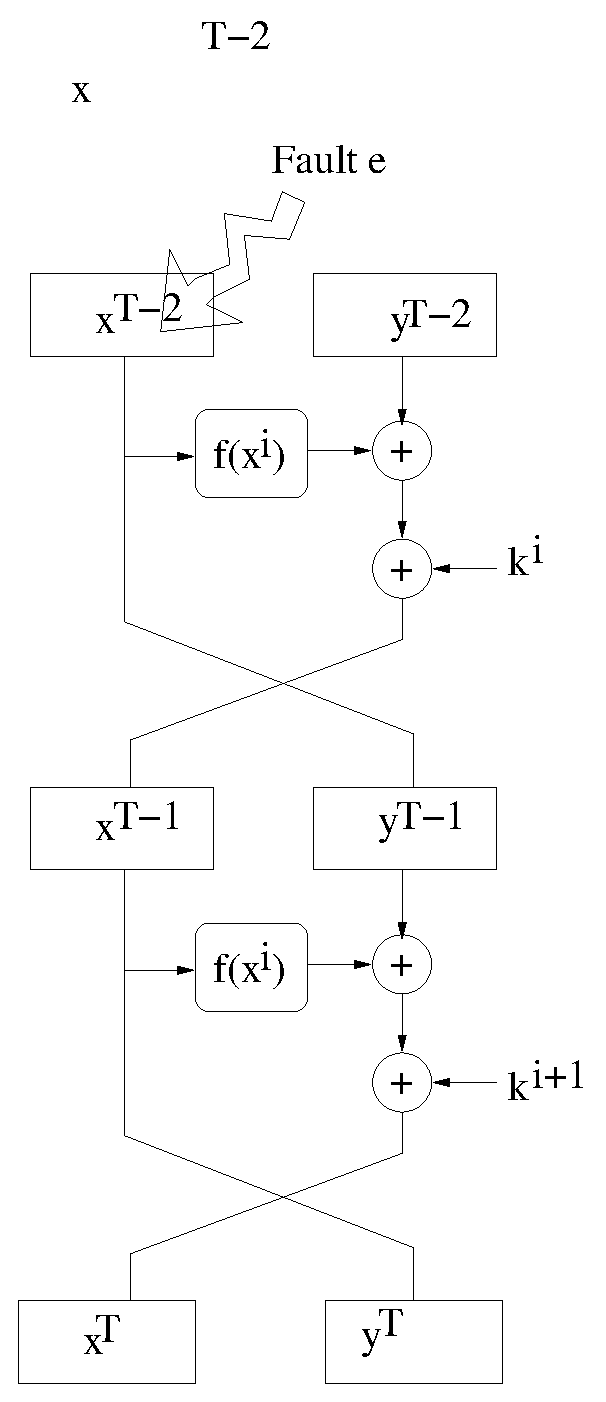
\includegraphics[width=1.5in]{DES}
%\epsfig{file= Images/isgreater.jpg, width=3.0in}
\caption{The last two rounds of a Fiestel Cipher}
\label{DES}
\end{figure}


\question
\begin{enumerate}
\item Define \textbf{uniqueness}, \textbf{uniformity} and \textbf{reliability}
metrics for a  PUF with suitable mathematical expressions. Which of these
parameters might be improved by addition of extra circuitry? \marks{5}
\item Suppose the truth tables of three instances of an 4-bit \emph{Arbiter PUF} 
circuit were found to be identical to those of AND4, NOR4 and XOR4 respectively.
Calculate the \emph{uniformity} and \emph{uniqueness} metrics. \marks{8}
\item Comment on the acceptability of the above PUF, by comparing the obtained
metric values with the ideal values. \marks{2}
\end{enumerate}

 


\question
\begin{enumerate}
\item Show that for an $n$-bit APUF circuit, determining the response for an
arbitrary challenge is the same as solving a linear separation problem in
$n$-dimensional space. \marks{8}
\item Suppose the \{$p$, $q$, $r$, $s$\} delay values (in arbitrary units) 
for the stages of an $4$-bit APUF are: \{\{22, 23, 17, 20\}, \{15, 14, 13, 9\}, 
\{20, 21, 22, 25\}, \{10, 12, 13, 16\}\}. Determine the direction
of a vector normal to the separating hyperplane for this APUF. Symbols
have their usual meaning. \marks{5}
\item What are the advantages and the disadvantages of the \emph{Genetic Programming}
based model building methodology? \marks{2}
\end{enumerate}

\question 
\begin{enumerate}
\item Consider a fault tolerant design of MixColumn of AES using byte-level parity bits, where the irreducible polynomial is 
$m(x)=x^8+x^4+x^3+x+1$. The MixColumn is defined as:
\begin{center}  
$M=\begin{pmatrix}
    2  &  3 & 1 & 1\\
    1  &  2 & 3 & 1\\
    1  &  1 & 2 & 3\\
    3 & 1 & 1 & 2\\
  \end{pmatrix}$
\end{center}
The input column is denoted by the vector: $(s_{0,j},s_{1,j},s_{2,j},s_{3,j})^T$. Also $p_{i,j}$ is the parity bit associated for the byte $s_{i,j}$ and $s_{i,j}^{(7)}$ is the most significant bit of $s_{i,j}$. Prove that the parity bits are transformed as follows:

\begin{eqnarray*}
p_{0,j} &=& p_{0,j} \oplus p_{2,j} \oplus p_{3,j} \oplus s_{0,j}^{(7)} \oplus 
s_{1,j}^{(7)}\\ 
p_{1,j} &=& p_{0,j} \oplus p_{1,j} \oplus p_{3,j} \oplus s_{1,j}^{(7)} \oplus 
s_{2,j}^{(7)}\\
p_{2,j} &=& p_{0,j} \oplus p_{1,j} \oplus p_{2,j} \oplus s_{2,j}^{(7)} \oplus 
s_{3,j}^{(7)}\\
p_{3,j} &=& p_{1,j} \oplus p_{2,j} \oplus p_{3,j} \oplus s_{3,j}^{(7)} \oplus s_{0,j}^{(7)}
\end{eqnarray*}
\marks{8}

\item Prof Faulty is interested to publish a paper on fault analysis of AES. He has the idea of inducing a random byte fault at the input of the last round of AES. Explain whether he can launch a successful attack. If yes, prove that the attack works. If not, suggest a suitable alteration of the fault model and explain how it works.
\marks{7}
\end{enumerate}

\end{questions}
\end{document}
